\documentclass[12pt, a4paper]{article}

\usepackage[utf8]{inputenc}
\usepackage[T1]{fontenc}
\usepackage{lmodern}
\usepackage[french]{babel}
\usepackage{amsmath, amssymb}
\usepackage{geometry}
\usepackage{graphicx}
\usepackage{float}
\geometry{a4paper, margin=1in}

\title{Modélisation Dynamique du Problème de Covoiturage par un Matching Temporel}
\author{Proposition de modèle dynamique}
\date{\today}

\begin{document}

\maketitle

\section{Introduction}
Ce document définit formellement le problème de covoiturage en utilisant une approche de matching dynamique et temporelle. Contrairement à un modèle statique, cette approche considère que les affectations entre passagers et conducteurs sont valides à des instants spécifiques, permettant une gestion plus fine et plus réaliste du problème.

La figure \ref{fig:reseau_cergy} illustre une instance typique du problème sur le réseau routier de Cergy-Pontoise, montrant la dispersion spatiale des passagers et des conducteurs au début d'une période d'observation.

\begin{figure}[H]
    \centering
    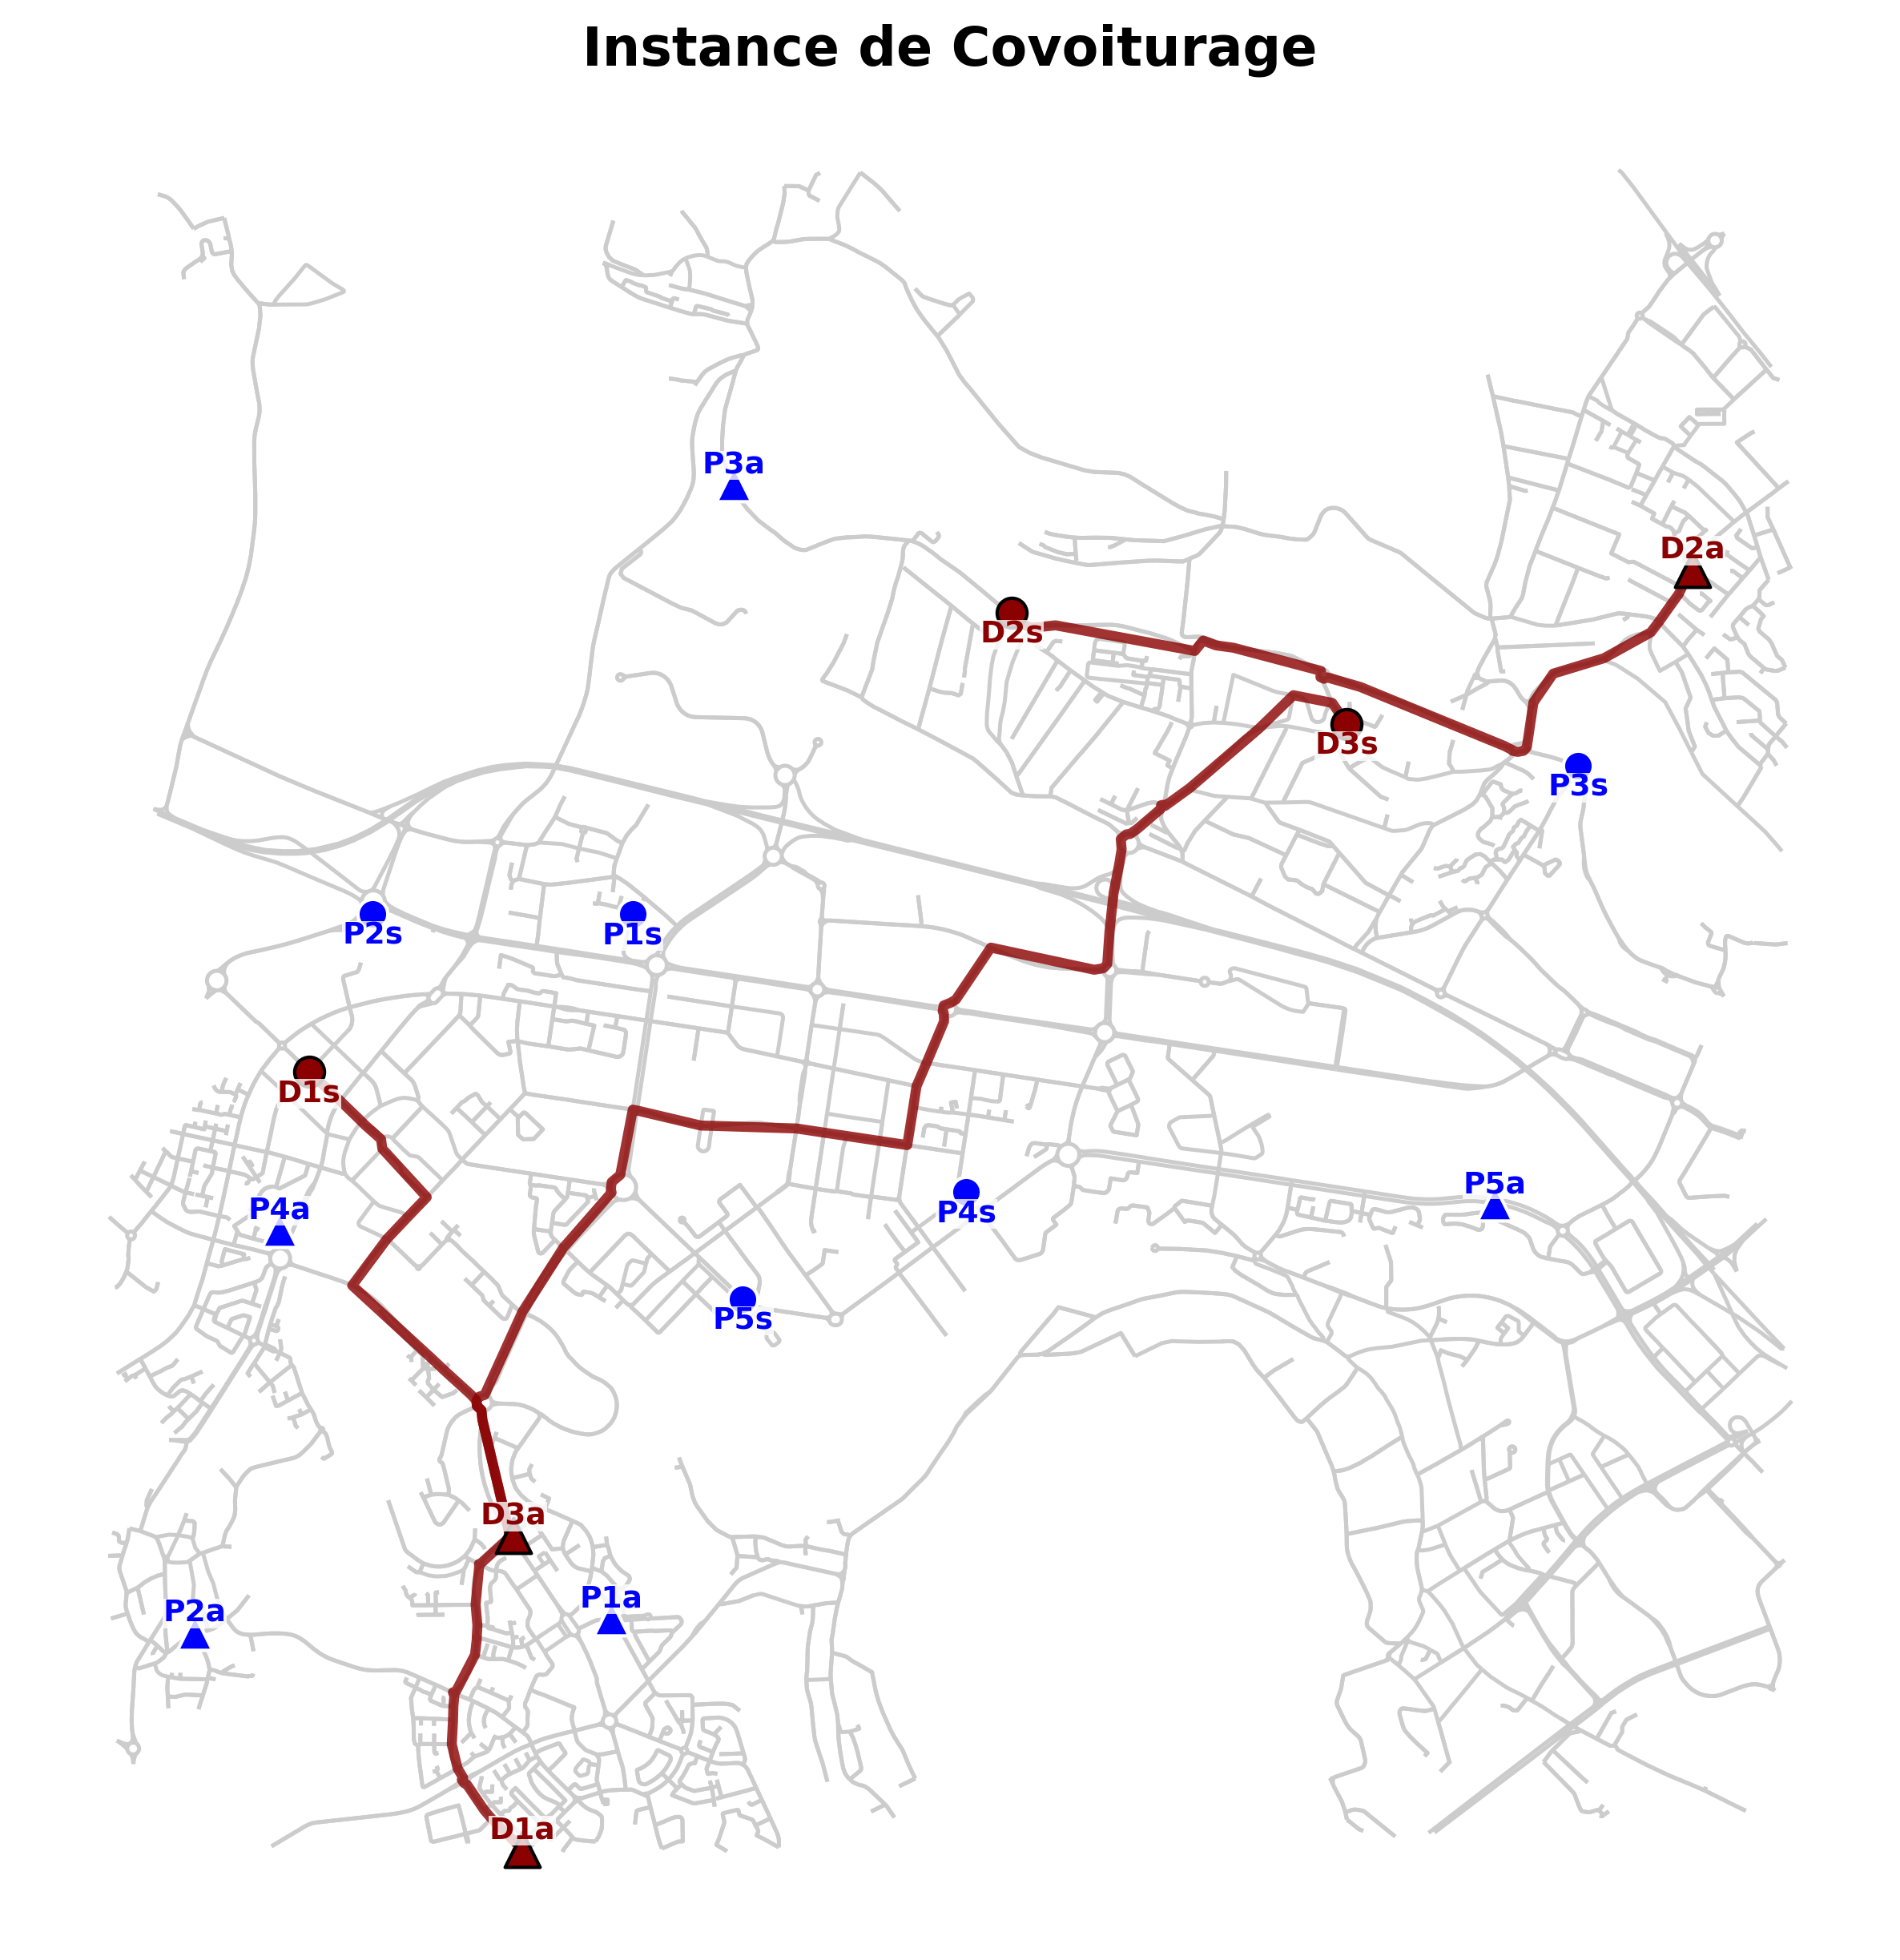
\includegraphics[width=0.7\textwidth]{map_covoiturage.png}
    \caption{Représentation spatiale du réseau routier et des agents (Passagers en bleu, Conducteurs en rouge) à Cergy.}
    \label{fig:reseau_cergy}
\end{figure}

\section{Définition des Concepts et Variables}

L'approche de modélisation est dynamique. L'affectation (ou \textit{matching}) est définie comme une fonction qui évolue au cours du temps.

\subsection{Les Agents et l'Intervalle de Temps}
Le problème met en jeu deux types d'agents :
\begin{itemize}
    \item $P = \{p_1, ..., p_n\}$, l'ensemble des passagers.
    \item $D = \{d_1, ..., d_k\}$, l'ensemble des conducteurs réels.
\end{itemize}
Pour modéliser le choix de marcher, on introduit un ensemble de véhicules "fantômes", $F = \{f_1, ..., f_n\}$, un pour chaque passager. L'ensemble étendu des véhicules est noté $D' = D \cup F$.

Le matching est effectué sur un intervalle de temps discrétisé $T$:
\begin{itemize}
    \item Soit $t_0$ l'instant initial d'observation du problème.
    \item Soit $\Delta t$ un pas de temps défini (ex: 1 minute).
    \item L'intervalle de temps est alors $T = \{t_0, t_0 + \Delta t, t_0 + 2\Delta t, \ldots, t_F \}$, où $t_F$ représente l'instant final du problème. Par convention, tous les instants définis dans ce modèle ($t_j^h, t_j^*, t_{d_i}^{max\_pickup}$, etc.) sont des éléments de $T$, tandis que les durées (notées $\Delta t$) sont supposées être des multiples du pas de temps.
\end{itemize}

\subsection{Désignations Temporelles}
Pour chaque passager $p_j$, nous définissons les variables temporelles suivantes :
\begin{itemize}
    \item $t^h_j$ : l'heure à laquelle le passager $p_j$ quitte la maison.
    \item $t^m_{i,j}$ : l'heure à laquelle le passager $p_j$ rencontre le conducteur $d_i$.
    \item $tt^{wo}_{i,j}$ : le temps de marche nécessaire pour que le passager $p_j$ rejoigne le point de rencontre avec le conducteur $d_i$ (temps d'accès).
    \item $tt^{wd}_{i,j}$ : le temps de marche nécessaire pour que le passager $p_j$ rejoigne sa destination finale depuis le point de dépose du conducteur $d_i$ (temps d'égress).
    \item $tt^c_{i,j}$ : le temps total de trajet en covoiturage pour le passager $p_j$ avec le conducteur $d_i$.
    \item $tt^M_j$ : le temps total de marche si le passager $p_j$ décide de marcher jusqu'à sa destination.
    \item $t^*_j$ : l'heure d'arrivée désirée du passager $p_j$.
    \item $ta_j$ : l'heure d'arrivée réelle à destination du passager $p_j$.
\end{itemize}

\subsection{La Fonction de Matching $\mu$}
Le matching est une application $\mu$ qui, pour chaque instant $t \in T$, associe un agent à un sous-ensemble d'autres agents.
$$ \mu: T \times (P \cup D') \to \mathcal{P}(P \cup D') $$
Cette fonction doit respecter les règles de cohérence suivantes pour tout $t \in T$, $p_j \in P$ et $d_i \in D'$ :
\begin{enumerate}
    \item \textbf{Point de vue du conducteur :} L'image d'un conducteur est l'ensemble des passagers qu'il transporte à l'instant $t$.
    $$ \mu(t, d_i) \subseteq P \quad \text{et} \quad |\mu(t, d_i)| < q_i $$
    où $q_i$ est la capacité totale du véhicule conduit par $d_i$ (incluant le conducteur). De plus, $\mu(t, d_i)$ doit être un ensemble de passagers compatibles entre eux. Pour un véhicule fantôme $f_j$, la capacité est définie comme $q_j = 2$ (incluant le passager).

    \item \textbf{Point de vue du passager :} L'image d'un passager est l'unique véhicule qui le prend en charge.
    $$ \mu(t^\prime, p_j) \subseteq D' \quad \text{et} \quad |\mu(t^\prime, p_j)| = 1, \quad \forall t^\prime \geq t_j^h $$
    Si $t < t_j^h$, le passager n'est pas encore actif dans le système et $\mu(t, p_j) = \emptyset$. De plus, si $t \geq t_j^h$ et $\mu(t, p_j) \neq \{f_j\}$, alors $\mu(t, p_j) \subset D$.

    \item \textbf{Condition de cohérence :} Un passager $p_j$ est dans l'ensemble d'un conducteur $d_i$ si et seulement si ce passager est assigné à ce conducteur.
    $$ p_j \in \mu(t, d_i) \iff \mu(t, p_j) = \{d_i\} $$
\end{enumerate}

\section{Le Schedule Delay Cost (SDC) : Analyse des Formes Possibles}
Le SDC mesure l'insatisfaction liée à la différence entre l'heure d'arrivée réelle ($ta_j$) et l'heure souhaitée ($t^*_j$). Plusieurs modélisations sont possibles selon le comportement recherché :

\subsection{Modèle Linéaire Symétrique}
$$ SDC(ta_j, t^*_j) = \alpha \cdot |t^*_j - ta_j| $$
L'avance et le retard sont pénalisés de la même manière.

\subsection{Modèle Quadratique}
$$ SDC(ta_j, t^*_j) = \alpha \cdot (t^*_j - ta_j)^2 $$
Pénalise très lourdement les grands écarts.

\subsection{Modèle Asymétrique Linéaire}
$$ SDC(ta_j, t^*_j) = \beta \cdot (t^*_j - ta_j)^+ + \gamma \cdot (ta_j - t^*_j)^+ $$
On considère généralement $\gamma > \alpha > \beta$ car être en retard est plus pénalisant (perte de productivité, rendez-vous manqué) qu'être en avance (temps d'attente passif).

\subsection{Modèle avec Pénalité Fixe de Retard}
$$ SDC(ta_j, t^*_j) = \beta \cdot (t^*_j - ta_j)^+ + \gamma \cdot (ta_j - t^*_j)^+ + \theta \cdot \mathbf{1}_{ta_j > t^*_j} $$
Où $\theta$ est un coût fixe subi dès que l'heure d'arrivée dépasse $t^*_j$, indépendamment de la durée du retard.

\section{Définition Analytique des Coûts}
Contrairement à la modélisation précédente où les coûts étaient représentés par une matrice statique $C_{i,j}$, nous définissons ici les coûts comme des fonctions dynamiques, dépendantes du temps et des agents impliqués. L'objectif est de capturer plus finement les différentes composantes de la "désutilité" associées à une affectation.

Nous distinguons principalement trois types de coûts : le coût de covoiturage, le coût de marche et un nouveau coût de compatibilité.

\subsection{Coût de Covoiturage $C^c(t, d_i, p_j)$}
Ce coût représente la désutilité encourue par le passager $p_j$ lorsqu'il est affecté au véhicule $d_i$ à l'instant $t$. Il intègre les aspects liés au temps de trajet et à la ponctualité.
$$
\begin{aligned}
C^c(t, d_i, p_j) &= \alpha^c \cdot tt^c_{i,j} + SDC(t, ta_j, t^*_j) \\
                 &\quad + \alpha^M \cdot (tt^{wo}_{i,j} + tt^{wd}_{i,j})
\end{aligned}
$$
où :
\begin{itemize}
    \item $tt^c_{i,j}$ est le temps total de trajet en covoiturage pour le passager $p_j$ avec le conducteur $d_i$.
    \item $SDC(t, ta_j, t^*_j)$ est le "Schedule Delay Cost" pour le passager $p_j$, mesurant l'insatisfaction liée à la différence entre l'heure d'arrivée réelle $ta_j$ et l'heure souhaitée $t^*_j$, et pouvant être fonction du temps $t$.
    \item $tt^{wo}_{i,j}$ et $tt^{wd}_{i,j}$ sont respectivement les temps de marche d'accès et d'égress pour le passager $p_j$ liés à son affectation à $d_i$.
    \item $\alpha^c$ et $\alpha^M$ sont les coups unitaires pour le transport motorisé et la marche.
\end{itemize}

\subsection{Coût du trajet marche $C^M(t, p_j)$}
Ce coût est encouru par le passager $p_j$ s'il choisit de ne pas covoiturer et utilise son véhicule fantôme $f_j$, ce qui implique qu'il marche jusqu'à sa destination. Ce coût est également dépendant du temps.
$$ C^M(t, p_j) = \alpha^M \cdot tt^M_j + SDC(t, ta_j, t^*_j) \footnote{L'inclusion du SDC ici reflète l'inadéquation potentielle entre la vitesse de marche et les contraintes horaires du passager : un retard devient inévitable si $t^h_j + tt^M_j > t^*_j$.} $$
où :
\begin{itemize}
    \item $tt^M_j$ est le temps total de marche du passager $p_j$ jusqu'à sa destination.
    \item $\alpha^M$ est un coefficient de pondération pour la marche.
\end{itemize}

\subsection{Coût de Compatibilité $C^{comp}(t, d_i, p_j, O(t, d_i))$}
Ce nouveau coût capture la "désutilité sociale" ou le frottement résultant de l'affectation d'un passager supplémentaire $p_j$ à un véhicule $d_i$ qui contient déjà un ensemble d'occupants. Il reflète la nécessité d'une harmonie entre les individus partageant le même espace et le même temps.

Nous définissons $O(t, d_i)$ comme l'ensemble des occupants du véhicule $d_i$ à l'instant $t$, incluant le conducteur $d_i$ lui-même et les passagers déjà présents.
Le coût de compatibilité $C^{comp}$ pourrait être modélisé de différentes manières, par exemple :
\begin{itemize}
    \item \textbf{Approche Binaire :} Un coût élevé (voire infini) si le passager $p_j$ est incompatible avec \textit{au moins un} occupant $x$ de $O(t, d_i)$. Zéro sinon. Cela correspond à la notion de "clique" où tous les membres doivent être compatibles.
    $$ C^{comp}(t, d_i, p_j, O(t, d_i)) = \begin{cases}
        \infty & \text{si } \exists x \in O(t, d_i) \text{ tel que } (p_j, x) \text{ incompatible} \\
        0 & \text{sinon}
    \end{cases} $$
    \item \textbf{Approche Continue :} Une somme des pénalités de compatibilité pour chaque paire $(p_j, x)$, où $x \in O(t, d_i)$.
    $$ C^{comp}(t, d_i, p_j, O(t, d_i)) = \sum_{x \in O(t, d_i)} \text{penalty}(p_j, x) $$
    où $\text{penalty}(\cdot, \cdot)$ est une fonction qui renvoie une valeur positive pour une incompatibilité et zéro pour une compatibilité.
\end{itemize}
Pour ce modèle, nous adopterons l'approche binaire pour les contraintes de compatibilité forte, en considérant un coût infini pour toute incompatibilité détectée. Les détails des critères d'incompatibilité (sociaux, préférences, etc.) seront définis comme des données d'entrée du problème.

L'objectif final de l'optimisation sera de minimiser la somme de ces coûts pour toutes les affectations sur l'ensemble de l'intervalle de temps $T$.

\section{Modélisation Décentralisée : Décision des Agents}

Cette section formalise le processus de décision individuelle des passagers. Dans ce modèle décentralisé, chaque passager $p_j$ résout son propre problème de minimisation de coût à chaque instant de décision $t \in T$.

\subsection{Espace des Options Admissibles}
Soit $\Phi(t, p_j) \subseteq D'$ l'ensemble des options de transport admissibles pour le passager $p_j$ à l'instant $t$. Un véhicule $d_i$ (réel ou fantôme) appartient à $\Phi(t, p_j)$ si et seulement si il satisfait l'ensemble des contraintes de faisabilité technique, temporelle et sociale :

\begin{enumerate}
    \item \textbf{Respect de la Capacité :}
    $$ |O(t, d_i) \cap P| + 1 <  q_i $$
    où $O(t, d_i)$ est l'ensemble des occupants du véhicule $d_i$ à l'instant $t$, et $q_i$ sa capacité.

    \item \textbf{Faisabilité Temporelle :}
    $$ \begin{cases}
        t^m_{i,j} \geq t^h_j + tt^{wo}_{i,j} \\
        t^m_{i,j} \leq t^{max\_pickup}_{d_i} \\
        ta_j \leq t^*_j + \Delta t^{tolerance}_j
    \end{cases} $$
    où :
    \begin{itemize}
        \item $t^m_{i,j}$ et $ta_j$ sont les heures de rencontre et d'arrivée estimées.
        \item $tt^{wo}_{i,j}$ est le temps de marche nécessaire pour rejoindre le point de rencontre.
        \item $t^{max\_pickup}_{d_i}$ est l'heure limite de prise en charge imposée par le trajet fixe du conducteur $d_i$.
        \item $\Delta t^{tolerance}_j$ est le retard maximal acceptable pour le passager $p_j$.
    \end{itemize}

    \item \textbf{Compatibilité Sociale :}
    $$ C^{comp}(t, d_i, p_j, O(t, d_i)) < \infty $$
\end{enumerate}

\subsection{Le Problème de Minimisation Individuel et Préférences}
Chaque passager $p_j$ choisit (ou se voit assigner) un instant de départ $t^h_j \in T$ représentant sa disponibilité initiale. À l'instant de décision $t \in T$ tel que $t = t^h_j$, le passager $p_j$ cherche à minimiser sa fonction de coût total $TC$ parmi les options disponibles à cet instant.

Ce comportement rationnel définit une \textbf{relation de préférence} $\succ_j$ sur l'ensemble des options admissibles $\Phi(t, p_j)$. Pour deux véhicules $d_1, d_2 \in \Phi(t, p_j)$, le passager préfère $d_1$ à $d_2$ si son coût associé est plus faible :
$$ d_1 \succ_j d_2 \iff TC(t, p_j, d_1) < TC(t, p_j, d_2) $$

La fonction de coût individuel total $TC$ est définie par :
$$ TC(t, p_j, d_i) = \begin{cases}
    C^c(t, d_i, p_j) + C^{comp}(t, d_i, p_j, O(t, d_i)) & \text{si } d_i \in D \\
    C^M(t, p_j) & \text{si } d_i = f_j
\end{cases} $$

Cette formulation garantit que chaque agent agit de manière rationnelle en classant les options selon son utilité propre, tout en respectant l'intégrité et les limites du système de covoiturage. Ces listes de préférences servent de base à l'algorithme de matching.

\section{Objectif : Recherche d'un Matching Stable}
Dans ce cadre de modélisation décentralisée, l'objectif principal est de déterminer un \textbf{matching stable} au cours du temps.

\subsection{Stabilité du Matching}
Un matching $\mu^*$ est dit stable si, pour chaque passager $p_j$ à son instant de départ $t = t^h_j$, l'affectation constitue un \textbf{équilibre stable}. Cela signifie qu'il n'existe aucune \textbf{paire bloquante} $(p_j, d_k)$ compatible qui aurait intérêt à se former en dehors du matching actuel.

Plus formellement, un matching $\mu^*$ est stable si, pour tout passager $p_j$ qui préférerait un conducteur $d_k$ à son conducteur assigné $d_i^* = \mu^*(t^h_j, p_j)$, le conducteur $d_k$ est dans l'une des situations suivantes :
\begin{enumerate}
    \item Il est déjà complet et préfère chacun de ses passagers actuels à $p_j$.
    \item Il est incompatible avec $p_j$ (ou l'un de ses occupants actuels l'est), rendant l'affectation inadmissible ($C^{comp} = \infty$).
\end{enumerate}

Cette condition garantit qu'à cet instant précis, aucun passager n'a d'incitation (ou de possibilité sociale) de modifier son choix pour une autre option. La stabilité du système est ainsi indissociable de la cohésion sociale des groupes formés.

Dans ce cadre dynamique, une fois le matching établi à $t^h_j$, le passager est considéré comme engagé dans son trajet. Un passager reste non matché (affecté à son véhicule fantôme $f_j$) seulement si aucune option de covoiturage n'est compatible à l'instant $t^h_j$ ou si le coût de la marche $C^M$ est inférieur à toutes les options de covoiturage réelles disponibles dans $\Phi(t^h_j, p_j)$.

\subsection{Efficacité et Performance Globale}
L'objectif secondaire est d'évaluer la qualité de cet équilibre par rapport à une solution globale théorique. Pour cela, on mesure l'efficacité globale du système par la somme des coûts de tous les passagers sur l'ensemble de l'horizon temporel $T$ :
$$ Z_{system} = \sum_{t \in T} \sum_{\{p_j \in P \mid t_j^h = t\}} TC(t, p_j, \mu^*(t, p_j)) $$
La comparaison entre ce coût global issu des décisions individuelles décentralisées et l'optimum théorique d'un modèle centralisé permet de quantifier la performance du système.


\section{Algorithme de Résolution : Gale-Shapley Adapté}
Pour déterminer le matching stable à un instant $t$ donné, nous utilisons une adaptation de l'algorithme de Gale-Shapley (acceptation différée), étendu au cas \textit{Many-to-One} (plusieurs passagers par véhicule).

\subsection{Construction des Listes de Préférences}
L'algorithme repose sur l'existence de listes de préférences établies par chaque agent :
\begin{itemize}
    \item \textbf{Préférences des Passagers :} Chaque passager $p_j$ classe les véhicules admissibles $d_i \in \Phi(t, p_j)$ par ordre croissant de son coût individuel total $TC(t, p_j, d_i)$. Son véhicule fantôme $f_j$ est inclus dans cette liste, marquant la limite d'acceptabilité du covoiturage.

    \item \textbf{Préférences des Conducteurs :} Chaque conducteur $d_i$ classe les passagers potentiels par ordre de \textbf{proximité}. Un passager est préféré s'il se situe spatialement plus près du trajet initial fixe du conducteur, minimisant ainsi l'impact indirect de la prise en charge.
\end{itemize}

\subsection{Fonctionnement de l'Algorithme}
Le processus se déroule de manière itérative jusqu'à l'obtention de la stabilité :
\begin{enumerate}
    \item \textbf{Phase de Proposition :} Chaque passager $p_j$ devenant disponible à l'instant $t$ (tel que $t = t^h_j$) propose de monter dans le véhicule qu'il préfère dans sa liste $\Phi(t, p_j)$ et qui ne l'a pas encore rejeté.
    \item \textbf{Phase d'Acceptation Différée :} Chaque conducteur $d_i$ reçoit les propositions des passagers. Il accepte temporairement les passagers les mieux classés dans sa liste de préférences, dans la limite de sa capacité $q_i$. Les autres passagers sont rejetés.
    \item \textbf{Terminaison :} L'algorithme s'arrête lorsqu'aucun passager n'a plus de proposition à formuler. Les passagers n'ayant pas trouvé de conducteur réel sont affectés à leur véhicule fantôme $f_j$.
\end{enumerate}
Ce mécanisme garantit l'obtention d'un matching stable au sens de l'équilibre de l'utilisateur.

\subsection{Théorème de Stabilité et Démonstration}
Pour que la stabilité du matching soit garantie mathématiquement dans ce cadre dynamique, nous posons les hypothèses fondamentales suivantes :
\begin{enumerate}
    \item \textbf{Hypothèse de trajet unique (Single-hop) :} Chaque passager $p_j$ ne peut être affecté qu'à un seul et unique véhicule $d_i \in D$ (ou son véhicule fantôme $f_j$) pour l'intégralité de son trajet.
    \item \textbf{Hypothèse d'engagement irréversible :} Une fois le matching établi à l'instant de départ $t^h_j$, le passager est considéré comme engagé. Il ne peut plus modifier son choix ni être sollicité par d'autres conducteurs lors des pas de temps ultérieurs $t > t^h_j$.
    \item \textbf{Hypothèse de trajet fixe des conducteurs :} Chaque conducteur $d_i$ suit un itinéraire prédéfini et invariant. Le covoiturage n'est autorisé que si la prise en charge et la dépose du passager s'effectuent sur cet itinéraire (ou dans les limites de détour acceptables $\Phi$).
    \item \textbf{Hypothèse d'information parfaite locale :} À chaque pas de temps $t$, le système possède une connaissance exhaustive de l'ensemble des passagers actifs $P_{actifs}(t)$ et de la capacité résiduelle de tous les véhicules $D'$.
\end{enumerate}

\textbf{Théorème 1 (Existence et Stabilité) :} Sous les hypothèses précédentes, pour toute instance du problème de covoiturage dynamique définie à l'instant $t$, il existe au moins un matching stable $\mu^*(t, \cdot)$ au sens de Gale-Shapley (absence de paires bloquantes compatibles).

\textbf{Démonstration :} La preuve de l'existence d'un tel équilibre repose sur le mécanisme de l'algorithme d'acceptation différée décrit précédemment. Procédons par un raisonnement par l'absurde pour démontrer la stabilité :

Supposons qu'à l'issue de la procédure de matching, il existe une paire bloquante $(p_j, d_k)$ compatible telle que le passager $p_j$ préfère le conducteur $d_k$ à son affectation actuelle, et que $d_k$ préfère $p_j$ à au moins un de ses passagers actuels (ou dispose d'une place libre).
\begin{enumerate}
    \item Selon la règle de proposition (Phase 1), chaque passager propose ses services aux conducteurs par ordre de préférence décroissant.
    \item Puisque $p_j$ préfère $d_k$ à son conducteur actuel, il a nécessairement formulé une proposition à $d_k$ avant d'être accepté par son conducteur final.
    \item Si $p_j$ n'est pas avec $d_k$ à la fin, c'est que le conducteur $d_k$ l'a rejeté (immédiatement ou par éviction ultérieure en Phase 2).
    \item Or, un conducteur ne rejette un candidat que s'il a déjà rempli sa capacité résiduelle $q_k(t)$ avec des passagers qu'il \textbf{préfère strictement} (critère de proximité).
    \item Par conséquent, à la fin de la procédure, le conducteur $d_k$ est complet et tous ses passagers sont mieux classés que $p_j$.
\end{enumerate}
L'hypothèse de départ est donc contredite : il ne peut exister de paire bloquante compatible. Le matching obtenu est stable.

\subsection{Pseudo-code de l'Algorithme Dynamique}
L'algorithme de matching est exécuté de manière itérative sur l'ensemble de l'intervalle de temps $T$ pour tenir compte de l'arrivée progressive des passagers.

\begin{itemize}
    \item[] \textbf{Pour chaque pas de temps $t \in T$ :}
    \begin{enumerate}
        \item \textbf{Identification des nouveaux passagers :}
        $$ P_{actifs}(t) = \{p_j \in P \mid t = t^h_j \} $$

        \item \textbf{Mise à jour des capacités disponibles :}
        Pour chaque conducteur $d_i \in D$, la capacité résiduelle $q_i(t)$ est calculée en soustrayant le nombre de passagers déjà présents dans le véhicule (matchés lors des pas de temps précédents et dont le trajet n'est pas terminé).
        \item \textbf{Matching Stable Local (Gale-Shapley) :}
        Appliquer Gale-Shapley pour l'ensemble $P_{actifs}(t)$ vers $D'$ avec les capacités $q_i(t)$ :
        \begin{itemize}
            \item Les passagers de $P_{actifs}(t)$ classent les options selon $TC$.
            \item Les conducteurs classent les nouveaux candidats selon la \textit{proximité}.
            \item Les propositions et acceptations différées sont effectuées jusqu'à stabilité.
        \end{itemize}

        \item \textbf{Mise à jour de l'état $\mu^*(t, \cdot)$ :}
        Les nouvelles affectations sont enregistrées et les passagers matchés sont retirés de la liste des candidats pour les pas de temps futurs.
    \end{enumerate}
\end{itemize}

\section{Discussion et Perspectives : Vers un Modèle Multi-Sauts}
La modélisation présentée dans ce document permet d'obtenir un matching stable et robuste pour des trajets simples. Cependant, l'atteinte de cette stabilité repose sur des hypothèses restrictives qui limitent l'optimalité globale du système.

\subsection{Limites du Modèle Actuel}
Les principales limites identifiées sont liées à la rigidité du processus de décision :
\begin{itemize}
    \item \textbf{Absence de correspondances :} L'hypothèse Single-hop interdit à un passager d'utiliser plusieurs véhicules successifs. Cela pénalise les trajets de longue distance où aucun conducteur unique ne couvre l'intégralité du besoin.
    \item \textbf{Engagement précoce :} L'hypothèse d'engagement irréversible empêche toute renégociation du trajet. Un passager déposé à un point intermédiaire est contraint de finir son trajet à pied, même si une option de covoiturage plus avantageuse devient disponible après son départ initial.
\end{itemize}

\subsection{Perspective : Le Modèle Multi-Sauts (Multi-Hop)}
Pour lever ces verrous, une extension naturelle de ce travail consiste à modéliser le problème comme un \textbf{matching multi-sauts}. Dans ce cadre, l'algorithme de Gale-Shapley ne serait plus appliqué uniquement à l'instant de départ initial $t^h_j$, mais de manière récursive.

\textbf{Principe de l'extension :}
Dès qu'un passager est déposé par un premier conducteur $d_1$, à l'instant $t = t^m_{1,j} + tt^c_{1,j}$, il est ré-injecté dans l'ensemble des passagers actifs $P_{actifs}(t)$. Son nouvel instant de disponibilité devient $t^h_j = t^m_{1,j} + tt^c_{1,j}$ et son point d'origine est mis à jour à sa position de dépose actuelle. Sa liste de préférences est alors recalculée dynamiquement pour le segment restant vers sa destination finale.

Cette approche transformerait le problème de matching en un problème de \textbf{recherche de chemin dynamique} dans un réseau d'opportunités de covoiturage, ouvrant la voie à une efficacité systémique bien supérieure, au prix d'une complexité algorithmique accrue et d'une gestion plus fine des temps de transfert.

\end{document}
